\documentclass{standalone}
\usepackage{tikz}
\usepackage{bbold}
\usepackage{tikz-network}

\begin{document}
\begin{minipage}[c]{0.2\textwidth}
\centering
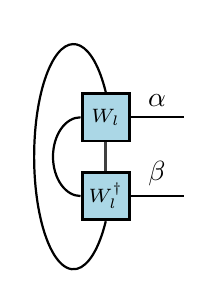
\begin{tikzpicture}
    % Main vertices (circles)
    \Vertex[x=0, y=0, label=$W_l$, shape=rectangle]{A}
    \Vertex[x=0, y=-1, label=$W_l^\dagger$, shape=rectangle]{B}
    \Edge[lw=1pt](A)(B)
    \draw[thick] (A) -- (1, 0) node[midway, above] {$\alpha$};
    \draw[thick] (B) -- (1, -1) node[midway, above] {$\beta$};
    \draw[thick] (0, 0.32) arc[start angle=35, end angle=325, x radius=0.5, y radius=1.43];
    \draw[thick] (-0.32, 0.0) arc[start angle=90, end angle=270, x radius=0.35, y radius=0.5];
\end{tikzpicture}
\end{minipage}
\begin{minipage}[c]{0.05\textwidth}
\centering
$=$
\end{minipage}
\begin{minipage}[c]{0.1\textwidth}
\centering
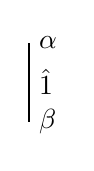
\begin{tikzpicture}
    \draw[thick] (0,0) -- (0, 1) node[midway, right] {$\hat{\mathbb{1}}$} node[at end, right] {$\alpha$} node[at start, right] {$\beta$};
\end{tikzpicture}
\end{minipage}
\end{document}